\scanpage{64}
\mspage{63}
% E: text|upper left|Pour les circuits fondamentaux
Pour les circuits fondamentaux sur $X$, \unsure{qui est|qui sont} de deux espèces

 a) \inserted{\uline{demi}} Circuit autour d'une \deleted{\unsure{droite}} \inserted{composante} exceptionnelle de $K$ (en la traversant une fois), soit $\ell_{D_i}$ le circuit correspondant à la pseudodrte $D_i\in\Sigma$. On trouve
% E: display|left upper middle|u(ell_D_i) translation par n-1
\[u(\vec\ell_{D_i})=\text{translation par }n-1\]
% E: text|left middle|dans le sens de l'orientation
(dans le sens de l'orientation de la portion \unsure{rect\textsuperscript{g}|rel.} $D$ voisine de $D_i$), valeurs des caractères fondamentaux
% E: display|left middle|chi_X(ell_D_i)=+1
\[\chi_X(\ell_{D_i})=+1,\quad\chi_s(\ell_{D_i})=\deleted{\unsure{+1}}(-1)^{n-1},\quad\deleted{\chi_c(\ell_{D_i})=1}\]
% E: text|lower left|b Demi-circuit autour d'un pt
b) Demi-circuit autour d'un pt de $X$ (qui peut être soit dans une face, soit dans un côté, soit \inserted{être} un sommet). La \deleted{point} \unsure{fibre} de ce point dans $\operatorname{Pol}(D)$ reste fixe par $u(\ell)$, qui est de signe $-1$, donc on trouve toutes les symétries, donc
% E: drawing|left margin beside b|double vertical emphasis
\figure{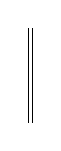
\begin{tikzpicture}[x=.2cm,y=.4cm]\draw (0,0)--(0,3);\draw (.25,0)--(.25,3);\end{tikzpicture}}
% E: display|lower left|u_D pi_1(X F_D) to Aut(F_D)
\[u_D:\pi_1(X,F_D)\longrightarrow\operatorname{Aut}(F_D)\]
% E: text|bottom left|est surjectif ouf
est \uline{surjectif}. ouf!
% E: text|upper right|Il semble que le caractère chi_c soit trivial
$*$ Il semble que le caractère $\chi_c$ soit \uline{trivial}! En effet, si pour une p.r. $D$ donnée, on désigne par $\mathrm{sing}_D$ (``singularité de $D$'') le nb de sommets de $\Sigma$ qu'elle contient, je dis que pour un chemin $c$ qui va de $D$ en $D'$, on a
% E: display|right upper middle|par c congruent sing_D' minus sing_D
\[\unsure{\mathrm{par}}\,c\equiv\mathrm{sing}_{D'}-\mathrm{sing}_D\qquad(2)\]
% E: text|right middle|donc parité paire si D=D'
(donc parité = \uline{paire} si $D=D'$!)
On est ramené au cas où $c$ est de longueur $1$, auquel cas cette formule est triviale. (en se rappelant que pour le franchissement \deleted{d'une \unsure{di.}} un ``balayage'' au dessus d'une \deleted{\unsure{droite}} $D_i\in\Sigma$, la parité est $2$.

Donc finalement, \uline{on trouve}
% E: display|lower right|chi_Xcal=chi_X
\[\boxed{\chi_{\mathcal X}=\chi_X}\]
% E: text|bottom right|il n'y a pas d'autres caractères
il n'y a pas d'autres caractères rigides que ceux provenant de $\mathbb D_2$!
